

\begin{abstract}

We present ColorSplit, an exact algorithm for counting the solutions Q(n) of the n-queens problem, and use it to compute the previously unknown value Q(28) = 2,564,269,152,506,723,832 in 436 hours on a single GPU (Section 8). The algorithm rests on one observation: queens on white squares never attack queens on black squares along a diagonal, so every solution splits into a white part and a black part that interact only through rows and columns (Section 3). For each set R of rows given to the white queens, the white placements are tabulated by their column set C, and each black placement on the remaining rows is matched by a single table lookup at the complementary column set (Sections 3 and 5).

We add a parity law that discards about 80\% of the row sets (Lemma 1), the board symmetries acting on row sets, a weighted transposition symmetry, early pruning on half of the key (Section 5), and a compact table indexed by combinatorial rank (Section 6). In our measurements the cost grows roughly as the square root of Q(n) times 2$^{n}$, compared with about Q(n) for backtracking (Sections 3 and 8). On one CPU core Q(21) takes 21 minutes, about 4 ns per solution, against an estimated 15 hours for symmetric bitmask backtracking (Section 8). On one NVIDIA RTX PRO 6000 Blackwell GPU, Q(24), Q(25) and Q(26) take 21 minutes, 1.75 hours and 13.4 hours; the fastest GPU solver we found in the literature needed 2.5 days on eight RTX 5090 GPUs for Q(26) (Section 2).

All our results up to n = 27 agree with OEIS A000170, and per-chunk partial sums agree exactly between independent CPU and GPU implementations wherever we compared them (Section 7). On one GPU we recomputed Q(27) = 234,907,967,154,122,528 in 62 hours of computation, against 28.4 days on eight GPUs in 2025, and computed Q(28) in 436 hours (Section 8). Q(28) passes every check we made: all 4096 partial sums are present and add up exactly, the total is divisible by 4, it continues the growth of Q(n) smoothly, and a random sample of 50 chunks, each recomputed with the table on both colors, agrees exactly (Section 7). All partial sums are published, so any part of the result can be recomputed independently.

This research was done with the help of Claude, an AI model by Anthropic. The research direction and the main ideas are the author's; Claude implemented and tested them, proposed some of the implementation techniques and drafted the text; the author ran all computations for n ≥ 22 (Section 11).

\end{abstract}
\section{Introduction}

The number Q(n) of ways to place n non-attacking queens on an n × n board was known only up to n = 27, and the first computations of the last values took months to years of specialized computing. No closed formula is known, and Q(n) grows like (0.143 n)$^{n}$ [Simkin 2023]. Near n = 27 it grows by a factor of about 10 per step, so a method that visits solutions one by one slows down by that factor with every step of n.

As far as we know, the recent record values were all obtained by faster enumeration of solutions. Q(24) came from a PC cluster in 2004 [Kise et al. 2004], Q(25) from grid computing in 2005 at a cost of about 53 CPU-years [OEIS A000170], Q(26) from an FPGA cluster in 2009 after nearly ten months, and Q(27) from FPGAs again in 2016 [Preußer and Engelhardt 2017]. In 2025 a GPU solver recomputed Q(26) in 2.5 days and Q(27) in 28.4 days on eight RTX 5090 GPUs, and estimated that the previous best GPU implementation would need over two decades and the FPGA approach over a decade for Q(28), while projecting about 11 months on eight RTX 5090 GPUs for its own solver [arXiv:2511.12009]. Section 2 lists these computations.

This paper takes a different route: it counts solutions without enumerating them one by one, and with it we compute the previously unknown value Q(28). Our contributions are:

\begin{enumerate}
\item{} The color decomposition: a solution is a white half and a black half joined by an exact key, so Q(n) is a sum of table lookups (Section 3).
\item{} Structural lemmas: a parity law on rows that makes the decomposition cheap, and facts about the diagonals that explain why the further splits we tried were slower (Section 4).
\item{} An algorithm, ColorSplit, combining the decomposition with symmetries, a weighted transposition, early pruning and a compact table (Section 5).
\item{} CPU and GPU implementations with resumable checkpoints and cross-checkable partial sums, released as open source (Sections 6 and 7).
\item{} The new value Q(28) = 2,564,269,152,506,723,832, computed in 436 GPU-hours on one GPU, with all 4096 partial sums published; measurements up to n = 28, including Q(27) in 62 GPU-hours against about 5450 GPU-hours for the 2025 GPU solver (Sections 7 and 8); and a list of ideas that did not help in our tests (Section 9).
\end{enumerate}

\section{Background and related work}

As far as we know, all record computations before this one counted solutions by depth-first backtracking with bitmasks. Occupied columns and both diagonal families are kept as machine words, so the free squares of the next row come from one AND-NOT, and the lowest free square from one bit trick [Richards 1997]. Exploiting the eight board symmetries by restricting the first queens and classifying solutions at the leaves saves up to a factor of 8 in principle and about 4.3 in our measurements (Section 8); we use such a solver ("BTSym") as our CPU baseline. Its cost per solution is roughly constant, about 170 ns on our test machine, because it visits every solution and many dead ends.

\begin{table}[htbp]\centering\small
\begin{tabularx}{\textwidth}{ll>{\raggedright\arraybackslash}X>{\raggedright\arraybackslash}p{0.25\textwidth}}\toprule
Value & Year & Method & Reported cost \\\midrule
Q(28) & 2026 & ColorSplit, color decomposition on GPU (this paper) & 436 hours on 1 × RTX PRO 6000 \\
Q(27) & 2025 & iterative DFS on GPU [arXiv:2511.12009] & 28.4 days on 8 × RTX 5090 \\
Q(27) & 2016 & FPGA cluster, Q27 project [Preußer and Engelhardt 2017] & about one year \\
Q(26) & 2025 & iterative DFS on GPU [arXiv:2511.12009] & 2.5 days on 8 × RTX 5090 \\
Q(26) & 2009 & FPGA cluster, Queens@TUD [Preußer et al. 2009] & about 10 months \\
Q(25) & 2005 & grid computing, INRIA ProActive [OEIS A000170] & about 53 CPU-years \\
Q(24) & 2004 & MPI on a PC cluster [Kise et al. 2004] & — \\
\bottomrule
\end{tabularx}
\end{table}

On the theory side (a survey of earlier results is [Bell and Stevens 2009]), Simkin proved that Q(n) = ((1 ± o(1)) n e$^{-c}$)$^{n}$ with c ≈ 1.942 [Simkin 2023], and Nielsen proved that Q(n) is divisible by 4 for all n ≥ 6 [Nielsen 2026], which we use as a sanity check. Completing a partial placement is NP-complete and counting completions is \#P-complete [Gent et al. 2017], which is consistent with our finding that cheap tests for dead branches catch few of them (Section 9). For a fixed number of queens the count is a quasi-polynomial in n [Chaiken et al. 2014], but this result does not cover the case of n queens on an n × n board.

Splitting the problem into parts that are solved separately and then combined is not new: divide-and-conquer was applied to constructing n-queens solutions by Abramson and Yung [Abramson and Yung 1989], and a counting program by Kluev splits the board into four quarters, solves each quarter separately and counts the compatible combinations [Kluev]. Such meet-in-the-middle splits along rows, into halves or quarters, leave parts that interact through both diagonal families, so matching them needs a disjointness test rather than a lookup by an exact key. In our earlier experiments the best such split, quarters joined through dictionaries, was about 1.7 times faster than symmetric backtracking at n = 18 to 21, with the same growth rate. Our split is along colors instead, which removes the diagonal interaction between the parts completely.

Splitting by color is classical for bishops. Arshon solved the problem of n non-attacking bishops by counting the placements on the black squares and on the white squares separately and combining the two counts [Arshon 1936]; the work was forgotten and later rediscovered by Kotěšovec [Kotěšovec 2013; Chaiken et al. 2020]. For bishops the two colors are fully independent. For queens they are coupled through rows and columns, and joining the two colors by the exact key of rows and columns, which is the basis of this paper, we have not found in the literature.

\section{The color decomposition}

Every n-queens solution is a white placement and a black placement that agree only on rows and columns. Call square (r, c) white when r + c is even. Both diagonal families keep r + c mod 2 fixed: along r − c = const and along r + c = const the parity of r + c never changes. Hence two queens of different colors can never share a diagonal.

Fix the set R of rows whose queen stands on a white square, and let C be the set of columns those white queens occupy. The black queens then fill exactly the remaining rows R$^{c}$ and columns C$^{c}$, where X$^{c}$ denotes the complement of X within \{0, …, n − 1\}; this complementarity is the only constraint between the two colors. Write W(R, C) for the number of non-attacking white placements with one queen in each row of R and column set C, and B(S, D) for the same count on black squares. Then:

\[Q(n) \;=\; \sum_{R \subseteq \{0,\dots,n-1\}} \; \sum_{|C| = |R|} W(R, C)\, B\bigl(R^{c}, C^{c}\bigr)\]

\begin{figure}[htbp]\centering
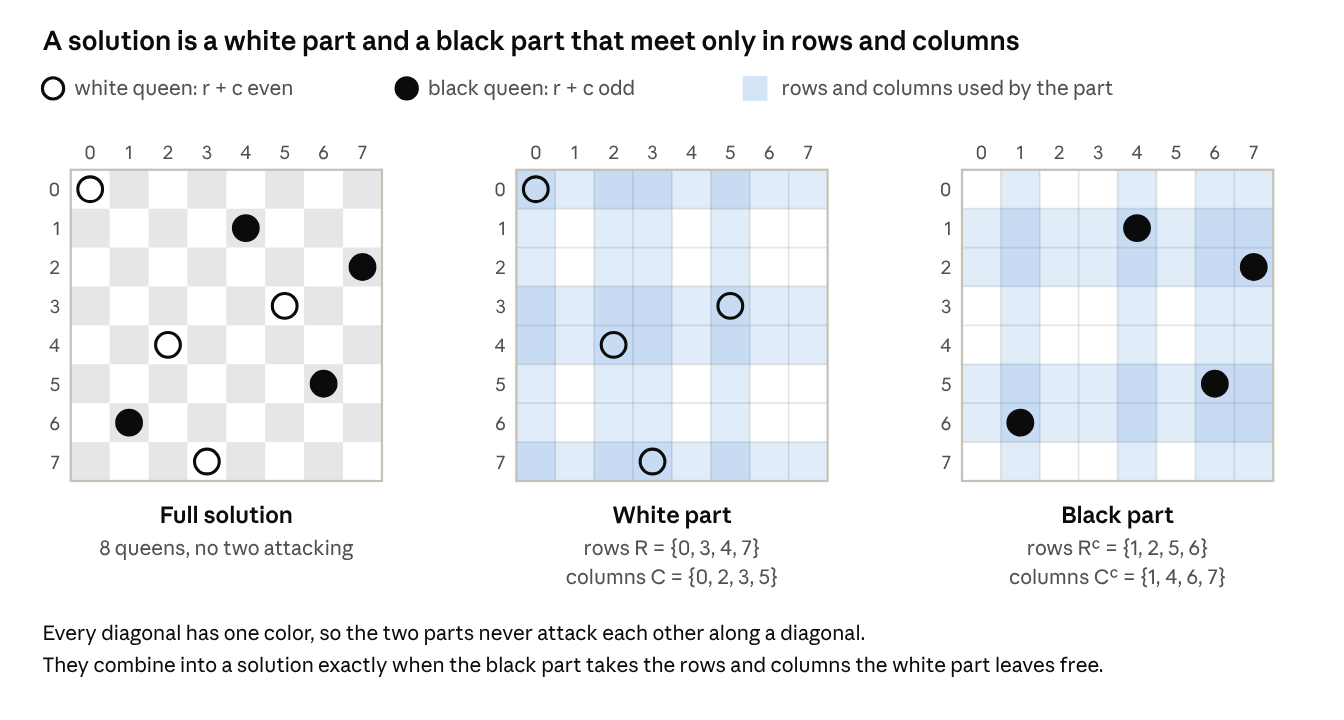
\includegraphics[width=\textwidth]{figs/fig1.png}
\caption{An 8 × 8 solution split by color}\label{fig:1}
\end{figure}

In Figure 1 the white part occupies the rows R and the columns C, and the black part fills exactly the remaining rows and columns; nothing else links the two parts.

The inner sum is a join on an exact key. For each R we enumerate the white placements once and count them in a table indexed by C. Then we enumerate the black placements on R$^{c}$, and each one adds the table entry at the complement of its column set: one lookup per black placement, no search. Solutions are never built; they are counted in bulk, which is why the cost per solution falls as n grows (Section 8).

The work per row set is about the number of white plus black placements, and both are far smaller than the number of solutions they combine into. Empirically the total cost behaves like the square root of Q(n) times 2$^{n}$, against about Q(n) for backtracking (Section 8, Figure 7).

\section{Structural lemmas}

The following facts make the decomposition cheap (Lemma 1) and describe the structure we met when we tried to refine it (Lemmas 2 to 4).

\textbf{Lemma 1 (parity law).} In every solution, the number of white queens in even rows equals the number in odd rows when n is even, and exceeds it by one when n is odd.

\emph{Proof.} Split the queens by the parities of row and column into the classes EE, EO, OE and OO. Each even row holds one queen, so EE + EO equals the number of even rows; each even column holds one queen, so EE + OE equals the number of even columns. These two numbers are equal, hence EO = OE. Using the odd rows, OE + OO equals the number of odd rows, so EE − OO = (even rows − EO) − (odd rows − OE) = even rows − odd rows, which is 0 or 1. The proof uses only rows and columns, so the law holds even for rooks.

\textbf{In plain words:} the white queens are always split evenly between the even and the odd rows (for odd n the even rows get one more), and the black queens exactly evenly. So when the algorithm chooses which rows get white queens, it only has to try choices with as many even rows as odd ones (one more even row for odd n).

Consequences. Only row sets R that satisfy the law can contribute. They make up the fraction

\[\binom{n}{\lfloor n/2 \rfloor} \Big/ \, 2^{n}\]

of all row sets: about 18\% at n = 20 and 15\% at n = 28. The number of white queens has the parity of n, so the number of black queens is always even. Within one table all keys have fixed numbers of queens in even and in odd columns, which the compact table of Section 6 exploits.

\textbf{Lemma 2 (no further linear laws for n = 9 to 32).} For every n from 9 to 32, the 0/1 incidence vectors of the solutions span an affine space of dimension (n − 1)$^{2}$, the same as all permutation matrices. So for these n, no weighting of squares (rings, sectors, crosses, blocks or any other) gives a sum that is the same in every solution, except combinations of row and column sums. For n ≤ 8 the rank is lower; at n = 8, for example, every solution has exactly four queens on white squares. We expect full rank for every n ≥ 9, but we have not proved it.

\emph{How we checked.} We computed ranks exactly modulo the prime 2$^{31}$ − 1; a rank modulo a prime is never larger than the rank over the rationals. For n = 9 to 13 we used all solutions, and for n = 14 to 32 between 230 and 1022 solutions found by randomized backtracking. The solution vectors are permutation matrices, so their rank is at most (n − 1)$^{2}$ + 1, and a set of solutions that reaches this rank settles the question for all of them (script tools/linear\_laws.py in the repository).

\textbf{In plain words:} besides the rule “one queen in every row and every column”, solutions obey no counting rule: no part of the board other than whole rows and columns, such as the center, the corners or the white squares, holds the same number of queens in every solution. At n = 8 there is one exception, four queens on the white squares in every solution; from n = 9 on there is none. So the search cannot use rules of this kind to stop a branch early.

\textbf{Lemma 3 (the diagonals connect each color).} For n ≥ 2, any two squares of the same color are joined by a path of diagonal steps.

\emph{Proof.} From a square in row r > 0, one of the two upward diagonal steps stays on the board, so every square is joined to a square of row 0; and the squares (0, c) and (0, c + 2) are joined through (1, c + 1).

Consequently, if the squares are split into classes so that no diagonal meets two classes, each color lies inside one class: the color split is the finest split of the squares with this property. Any split of the squares of one color, such as EE and OO for white or EO and OE for black, leaves parts that share diagonals, so they interact through diagonals as well as through rows and columns. In the splits of this kind that we tried, the join needed a disjointness test and was slower (Section 9). The lemma concerns splits of the squares only; it does not rule out decompositions of other kinds.

\textbf{In plain words:} a bishop can reach every square of its own color. So the two colors are the smallest pieces the board can be cut into without the pieces sharing a diagonal; any finer cut brings diagonal conflicts back.

\begin{figure}[htbp]\centering
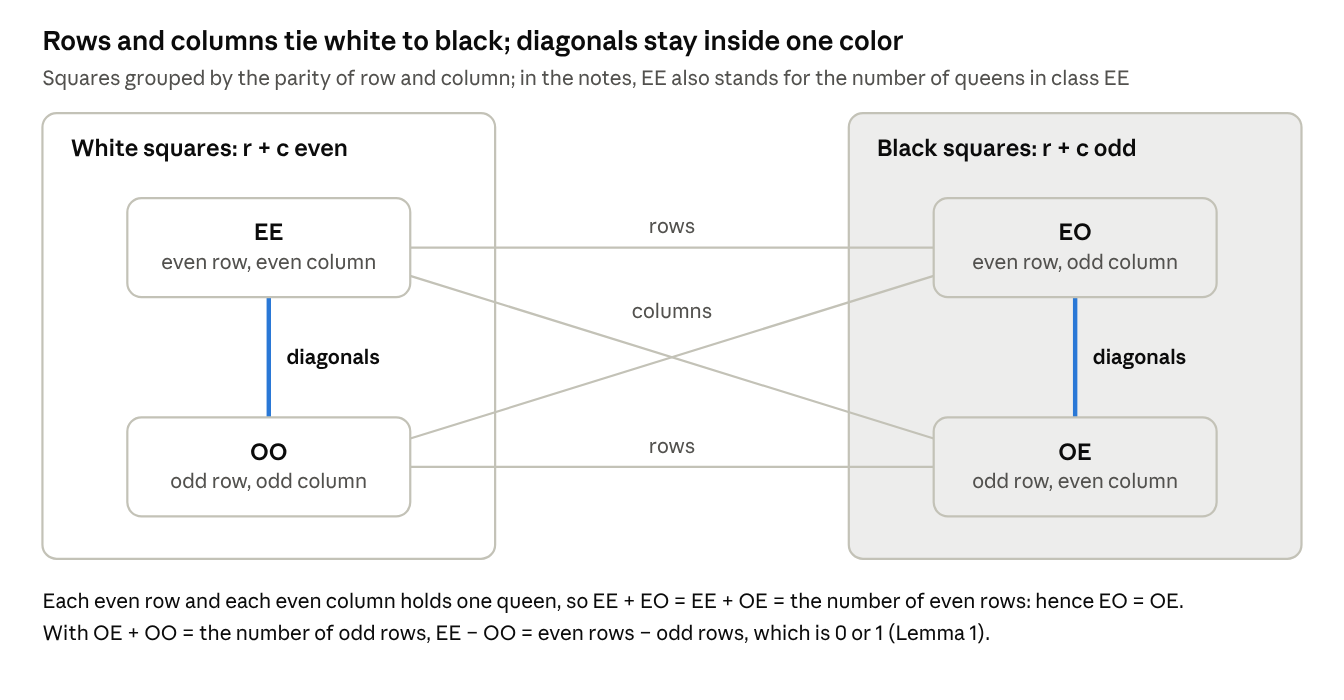
\includegraphics[width=\textwidth]{figs/fig2.png}
\caption{The four parity classes of squares and what links them}\label{fig:2}
\end{figure}

Figure 2 puts Lemmas 1 and 3 side by side: rows and columns link classes of different colors, which gives the parity law, while diagonals link only the two classes of one color.

\textbf{Lemma 4 (edge law).} Every solution has exactly three or four queens on the border, three exactly when a corner is occupied, and at most one corner can be occupied. This follows from rows 0 and n − 1 and columns 0 and n − 1 each holding one queen, and from any two corners sharing a row, a column or a diagonal. It is a useful sanity check; we have not found a way to use it for pruning.

\textbf{In plain words:} the top row, the bottom row, the left column and the right column each hold exactly one queen. A queen in a corner is counted twice, so the border holds four queens, or three when a corner is taken.

\section{The ColorSplit algorithm}

ColorSplit loops over the row sets R that satisfy the parity law and are canonical under the board symmetries, and for each one builds a table and probes it. The steps below each cut the work by a measured factor.

\textbf{Table and probe.} One color is enumerated by bitmask backtracking over its rows and its column sets are counted in a table; the other color is enumerated the same way and each complete placement adds the table entry of the complementary column set. The color with more rows goes into the table, which saves 5 to 15\% in our CPU measurements (when we recomputed a sample of Q(28) with the table forced to black, that side took much longer on the GPU, for reasons we do not yet understand, so we cannot claim that this saving holds on large boards; see Section 7).

\textbf{Symmetries on row sets.} Three board symmetries keep rows as rows: the left–right mirror, the top–bottom mirror and the half turn. Write rev(X) for a row or column set X read in reverse order. For even n the two mirrors swap the colors of the squares, and a solution with white rows R and white columns C becomes (Figure 3):

\begin{itemize}
\item{} after the left–right mirror: white rows R$^{c}$, white columns rev(C)$^{c}$;
\item{} after the top–bottom mirror: white rows rev(R)$^{c}$, white columns C$^{c}$;
\item{} after the half turn: white rows rev(R), white columns rev(C).
\end{itemize}

So R, R$^{c}$, rev(R) and rev(R)$^{c}$ contribute equally. Only the smallest member of each such orbit is computed, weighted by the orbit size. For odd n the mirrors keep the colors, and the orbit of R is \{R, rev(R)\}.

\begin{figure}[htbp]\centering
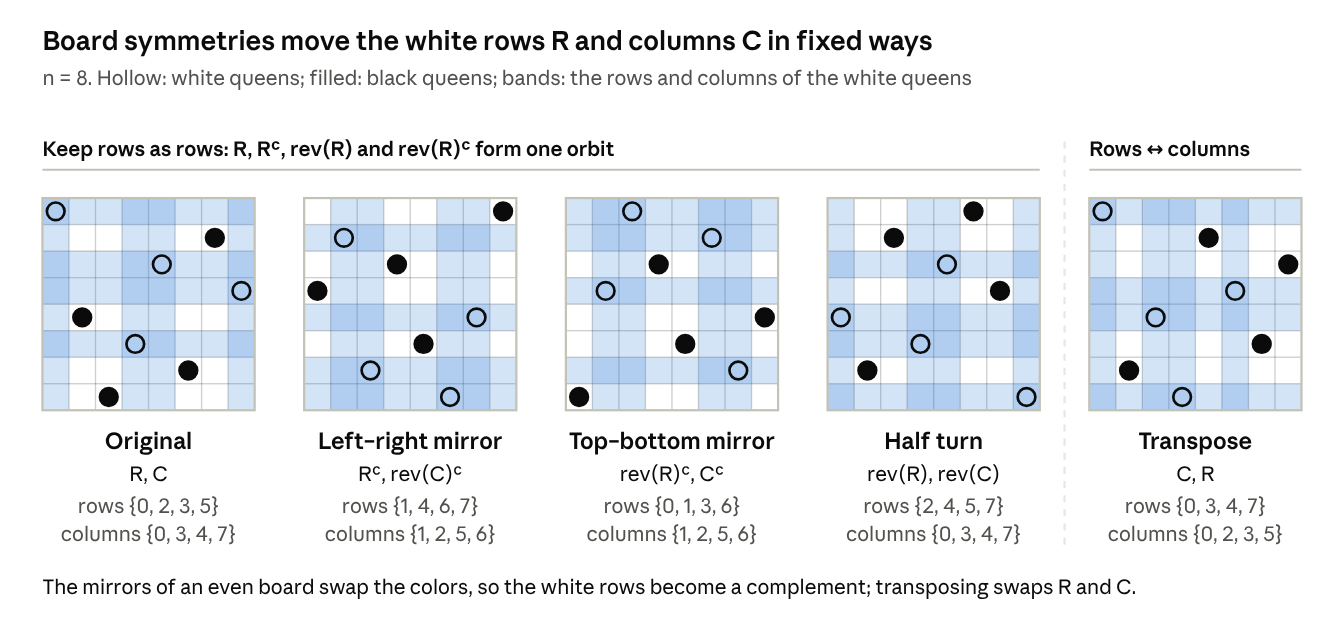
\includegraphics[width=\textwidth]{figs/fig3.png}
\caption{One solution under the board symmetries that keep rows as rows, and under transposition}\label{fig:3}
\end{figure}

In Figure 3 the white rows \{0, 2, 3, 5\} become \{1, 4, 6, 7\} = R$^{c}$ under the left–right mirror and \{0, 1, 3, 6\} = rev(R)$^{c}$ under the top–bottom mirror; the transpose swaps the roles of rows and columns.

For odd n the left–right mirror keeps R and maps C to rev(C), so W(R, rev(C)) = W(R, C). We use this inside each row set (Figure 4):

\begin{itemize}
\item{} The first queen of the first enumerated row goes only into the left half, where it is counted twice, or into the center column. In the center case the same restriction is applied to the second row.
\item{} On the table side, a placement counted twice stands for itself and its mirror image, so its count goes to the cell of min(C, rev(C)). A lookup at C returns half of that cell when C ≠ rev(C) and the whole cell otherwise, which is exactly W(R, C).
\item{} On the probing side the restriction is exact, because W(R, rev(C)) = W(R, C).
\end{itemize}

This nested mirror saves about 17\% on odd boards.

\begin{figure}[htbp]\centering
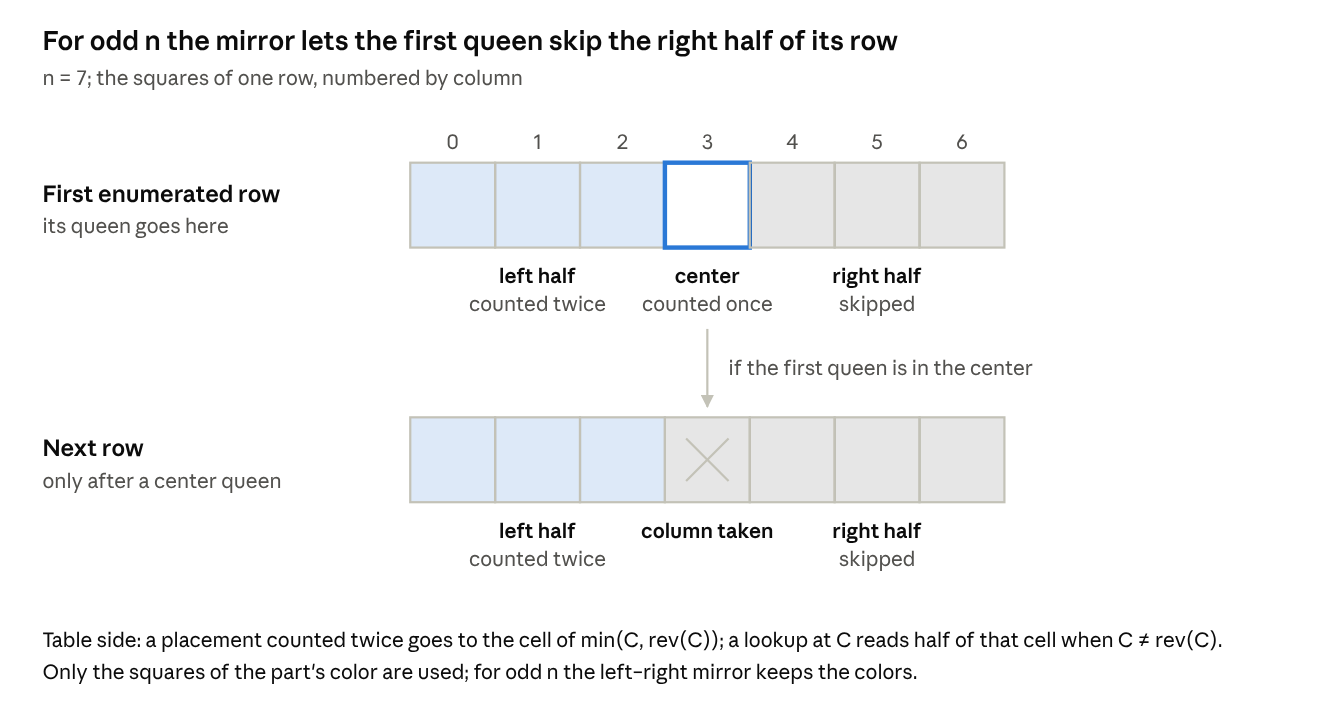
\includegraphics[width=\textwidth]{figs/fig4.png}
\caption{The nested mirror for odd n}\label{fig:4}
\end{figure}

Figure 4 shows where the first queen may stand: the right half of the row is never enumerated, because each placement there is the mirror image of one in the left half.

\textbf{Weighted transposition.} Transposing the board, that is, reflecting it in its main diagonal, moves a queen from (r, c) to (c, r). It keeps the colors of the squares and turns a solution with white rows R and white columns C into one with white rows C and white columns R (Figure 3, right). Write f(R, C) = W(R, C) · B(R$^{c}$, C$^{c}$) for one term of the sum; then f(C, R) = f(R, C). For R ≠ C the sum therefore contains each such value twice: once as the key C in the term of R, and once as the key R in the term of C. Computing it once and doubling it halves the work.

ColorSplit computes the term of each row set on its own, so the choice of which copy to keep must be a rule that each term can apply alone. We use an order. Let I be any function on subsets of \{0, …, n − 1\}, and give each pair the weight

\[\lambda(R,C) \;=\; \begin{cases} 2 & \text{if } I(C) > I(R),\\ 1 & \text{if } I(C) = I(R),\\ 0 & \text{if } I(C) < I(R). \end{cases}\]

The term of R keeps the keys that come after R in the order of I, with weight 2, drops those that come before it, and keeps ties with weight 1 (Figure 5). Transposition maps the pairs with I(C) < I(R) one to one onto those with I(C) > I(R), so

\[\sum_{R,\,C} f(R,C) \;=\; \sum_{R,\,C} \lambda(R,C)\, f(R,C).\]

Ties keep weight 1, so nothing is counted twice, whether or not I separates different orbits.

\begin{figure}[htbp]\centering
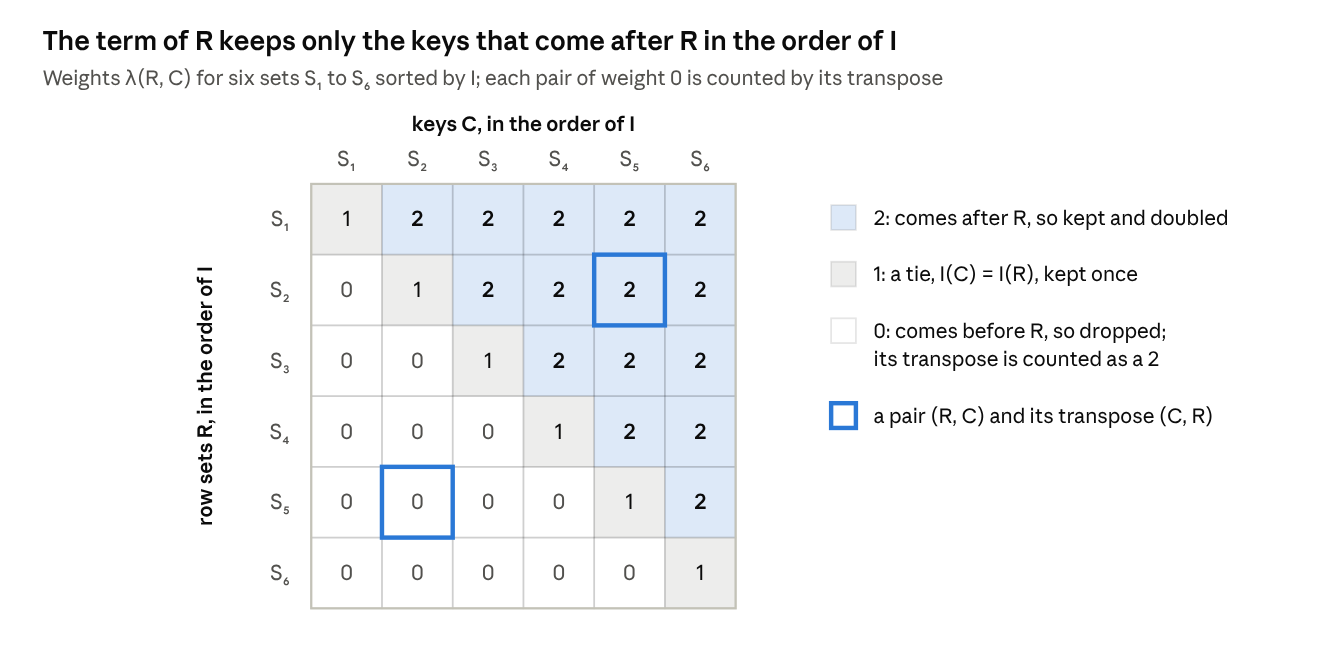
\includegraphics[width=\textwidth]{figs/fig5.png}
\caption{The weights λ: row sets against keys, both in the order of I}\label{fig:5}
\end{figure}

In Figure 5 every pair below the diagonal is dropped, and its transpose above the diagonal is counted twice in its place; the diagonal keeps weight 1.

To apply the identity to each orbit representative separately, I must also take the same value on all members of an orbit: it must be invariant under complement, rev and their composition for even n, and under rev for odd n. We take

\[\begin{aligned} n \text{ odd:}\quad & I(S) = \min\bigl(\mathrm{key}(S),\, \mathrm{key}(\mathrm{rev}\,S)\bigr), \qquad \mathrm{key}(S) = 2^{n}\,\mathrm{odd}(S) + \mathrm{even}(S),\\ n \text{ even:}\quad & I(S) = 2^{n} \min(u, v) + \max(u, v), \qquad u = h(\mathrm{odd}(S)),\;\; v = h\bigl(\mathrm{rev}(\mathrm{even}(S))\bigr), \end{aligned}\]

where odd(S) and even(S) are the bit masks of the odd and of the even elements of S, and h(x) is the smaller of x and its complement within the odd positions.

Any I gives the exact sum; the choice matters only for speed. The sum gets cheaper only if the placements of weight 0 are never enumerated, and our I lets the weight of a branch be decided before its last rows are placed (the early cut, below). In the code the weights are applied once per row set: after the table is built, every cell is multiplied by its λ and the keys of weight 0 are removed (Algorithm 2). A lookup at C then returns λ(R, C) · W(R, C).

\textbf{Early cut.} The early cut skips the table placements whose key would get weight 0. It relies on the colors: a white square has r + c even, so a white queen in an even row stands in an even column and one in an odd row in an odd column; for black queens it is the other way round (Figure 2).

The table color first enumerates its rows of the parity whose columns form the high part of I. Once those rows are filled, the columns of that parity are final: the queens still to come, in rows of the other parity, can only take columns of the other parity. For odd n the high part ⌊I(C)/2$^{n}$⌋ equals min(odd(C), odd(rev(C))) and is then known exactly. For even n it equals min(u, v), and only one of u and v is known, which gives an upper bound.

If this value is already below ⌊I(R)/2$^{n}$⌋, every completion of the branch has I(C) < I(R) and weight 0, and the branch is cut before its remaining rows are enumerated. With these weights the work halves for odd n and falls by a factor of about 1.4 for even n, where only an upper bound is known early.

\textbf{Half-key pruning.} The probing color uses the same property of the colors. Black enumerates its even rows first, whose black squares lie in odd columns; white, when black is in the table, enumerates its odd rows first, whose white squares also lie in odd columns. Once these rows are filled, the odd columns of the probing placement are final, and so is the odd-column half of the key it needs, the complement of its column set.

Before the remaining rows are enumerated, the probe checks this half against the set H of odd halves of all table keys of nonzero weight, built after the weights are applied (Algorithm 2). If no table key has this half, no completion of the branch can find a partner, and the branch is cut. Because the keys of weight 0 are left out of H, the weighted transposition makes this test cut more often. In the C version, switching the half-key pruning off makes the run about 1.2 times slower at n = 18 and 20 and 1.4 times slower at n = 19.

\textbf{Row order.} Within each parity class, rows are enumerated from the center outward. Central rows have the longest diagonals and constrain the others most, so dead ends appear earlier; this saves 10 to 20\% with no cost per node.

\begin{figure}[htbp]\centering
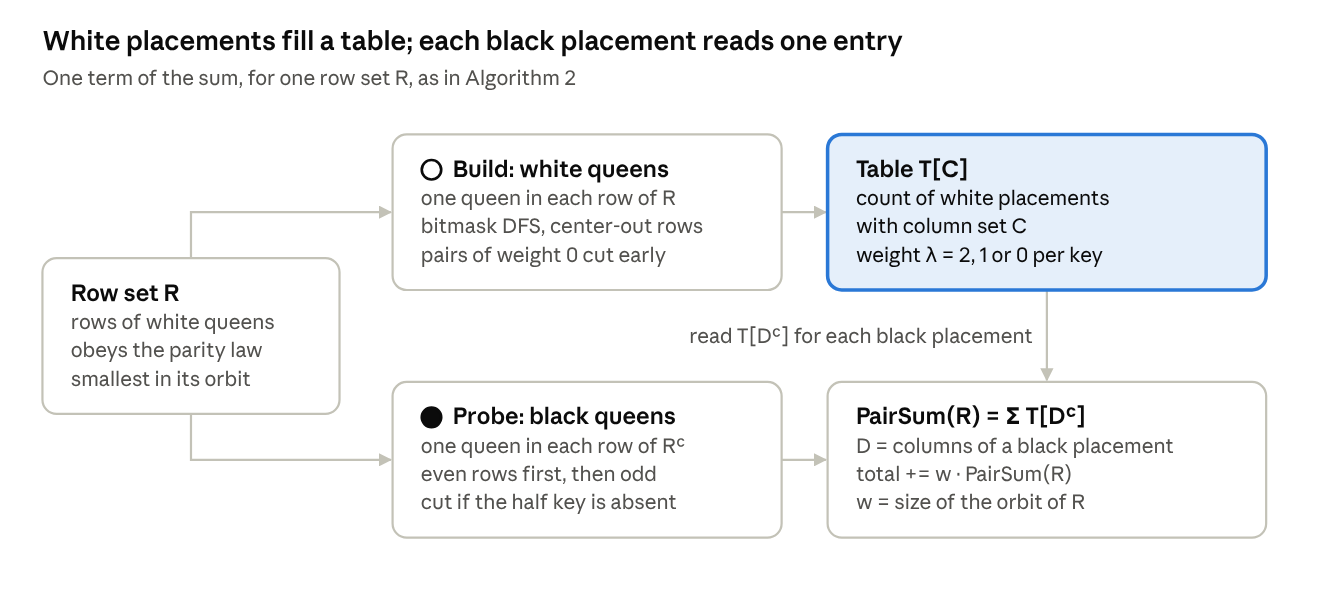
\includegraphics[width=\textwidth]{figs/fig6.png}
\caption{One term of the sum: build the table, then probe it}\label{fig:6}
\end{figure}

Figure 6 puts these steps together for one row set: the table is built once from the white placements, and every black placement then costs a single lookup.

\textbf{Exactness.} Together, these steps compute

\[Q(n) \;=\; \sum_{R\ \text{canonical}} w(R) \sum_{C} \lambda(R,C)\, f(R,C),\]

where R runs over the row sets that satisfy the parity law and are the smallest of their orbit, and w(R) is the orbit size. This is exact:

\begin{itemize}
\item{} the color identity of Section 3 gives Q(n) as the sum of f(R, C) over all pairs;
\item{} the transposition identity holds for any I;
\item{} every board symmetry maps a pair (R, C) to a pair (σR, σ′C) with f(σR, σ′C) = f(R, C), I(σR) = I(R) and I(σ′C) = I(C), so the inner sum is the same for all members of an orbit;
\item{} the mirror, the early cut, the half-key pruning and the choice of the table side change only how the inner sum is evaluated, not its value.
\end{itemize}

Section 7 lists tests that check each of these steps separately.

\subsection*{Pseudocode}

Algorithm 1 is the whole method; Algorithm 2 computes one term of the sum. As in Section 3, X$^{c}$ is the complement of a row or column set X within \{0, …, n − 1\}.

\begin{algobox}
\noindent\textbf{Algorithm 1.} ColorSplit(n)\par\smallskip
\begin{Verbatim}[fontsize=\small]
  total ← 0
  for each row set R ⊆ {0, …, n−1}:
      if R violates the parity law (Lemma 1): skip
      if R is not the smallest member of its symmetry orbit: skip
      w ← size of the orbit of R
      total ← total + w · PairSum(R)
  return total
\end{Verbatim}
\end{algobox}

\begin{algobox}
\noindent\textbf{Algorithm 2.} PairSum(R)\hfill{\small\itshape white queens in the table; the black-table side is symmetric}\par\smallskip
\begin{Verbatim}[fontsize=\small]
  T ← empty compact table;  compute I(R)

  // build: one white queen in each row of R
  for each white placement P on rows R (bitmask DFS, Algorithm 3):
      at the depth where the first parity class of rows is placed:
          if the known half of the columns already gives I(C) < I(R): cut branch
      C ← column set of P
      T[rank(C)] ← T[rank(C)] + 1

  // weights and half keys
  H ← ∅
  for each key C present in T:
      λ ← 2 if I(C) > I(R),  1 if I(C) = I(R),  0 otherwise
      T[rank(C)] ← λ · T[rank(C)]
      if λ > 0: H ← H ∪ { odd-column half of C }

  // probe: one black queen in each row of Rᶜ, even rows first
  s ← 0
  for each black placement Q on rows Rᶜ (bitmask DFS):
      at the depth where all even rows are placed:
          if the odd-column half of cols(Q)ᶜ is not in H: cut branch
      s ← s + T[rank(cols(Q)ᶜ)]
  return s
\end{Verbatim}
\end{algobox}

\begin{algobox}
\noindent\textbf{Algorithm 3.} One step of bitmask DFS at row r\par\smallskip
\begin{Verbatim}[fontsize=\small]
  free ← colorMask[r] AND NOT (cols OR (diag1 >> shift1(r)) OR (diag2 >> shift2(r)))
  while free ≠ 0:
      b ← free AND (−free)            // lowest free square, column c
      free ← free XOR b
      recurse with cols | b,  diag1 | bit(c − r + n − 1),  diag2 | bit(r + c)
\end{Verbatim}
\end{algobox}

\begin{algobox}
\noindent\textbf{Algorithm 4.} GPU thread block\par\smallskip
\begin{Verbatim}[fontsize=\small]
  for each row set R assigned to this block:
      thread 0: set up the rows of both colors and I(R);           barrier
      all threads: build the table, sharing the depth-4 prefixes
                   among the threads of the block;                barrier
      all threads: apply weights λ, mark half keys in shared memory; barrier
      all threads: probe, sharing the prefixes the same way,
                   and add local sums to the block sum;           barrier
      thread 0: atomically add w · (block sum) to its chunk total
      all threads: clear the table cells that were touched;       barrier
\end{Verbatim}
\end{algobox}

\section{Implementation}

We have a Java and a C implementation for CPUs and a CUDA implementation for GPUs; all three split the work into the same 4096 chunks of row sets. Chunk k holds the row sets R in [k · 2$^{n-12}$, (k + 1) · 2$^{n-12}$), and its partial sum is written to a checkpoint file. The format is shared, so a computation can be resumed by any implementation or split between machines. All three implementations are in the accompanying repository.

\textbf{Compact table.} By Lemma 1, all keys of one table have fixed numbers k$_{e}$ and k$_{o}$ of queens in the even and in the odd columns. Let n$_{e}$ and n$_{o}$ be the numbers of even and odd columns, and rank$_{e}$ and rank$_{o}$ the colex ranks of the even- and odd-column halves of a key. The key is stored at

\[\mathrm{index} \;=\; \mathrm{rank}_e \cdot \binom{n_o}{k_o} + \mathrm{rank}_o,\]

so the table has at most

\[\binom{n_e}{\lfloor n_e/2 \rfloor} \binom{n_o}{\lfloor n_o/2 \rfloor}\]

cells instead of 2$^{n}$: 16.5 times fewer at n = 19 and 22.8 times fewer at n = 28, where one table of 32-bit cells needs 47 MB instead of 1.07 GB. Counting the list of keys in use, a CPU thread needs about 12 bytes per compact cell, against 16 bytes per cell of the full table in our first version: 22 times less memory at n = 19 and 30 times less at n = 28. Cells are cleared through the list of touched keys, so no generation stamps are needed.

\textbf{CPU version.} Each thread owns a table and takes chunks from a shared counter. Bit compression for the rank uses the pext instruction where it is fast and a lookup otherwise. The C version is 15 to 30\% faster than Java on large boards; profile-guided optimization adds 2 to 5\%.

\textbf{GPU version.} Each thread block takes one row set at a time and keeps its table in global memory. The threads of the block enumerate the table color together, then filter by the transposition weight, mark the half keys in shared memory, enumerate the probing color and reduce the sum. Inside a block, work is shared by prefixes of depth 4: every thread enumerates the prefixes in the same order and processes every k-th one, where k is the number of threads.

The results for Q(25) to Q(27) in Section 8 come from the second version of this kernel; with 512 threads per block, tuning gave a factor of 1.25 over the first version at n = 23. A later version takes prefixes dynamically from a shared counter, keeps only the free squares and the chosen column per depth on the stack, and compresses bits with shifts and masks instead of table lookups. It also stops with an error if a table counter approaches 2$^{31}$, so that doubling by λ can never exceed 32 bits.

This later version gives the same chunk sums in CPU emulation and the known values Q(4) to Q(23) on the GPU, where it computes Q(23) in 80 seconds, against 157 seconds for the second version in the same session. On a batch of 32 chunks of Q(27) it reproduced the sums of our Q(27) run and took about 640 seconds, against 693 seconds for the second version: on large boards, where memory access dominates, the gain is only about 8\%. Our current version also hands the row sets to the blocks dynamically, the heaviest first. On the same batch it took 10.6 minutes while saving a checkpoint every 8 chunks, against 10.7 minutes with a checkpoint every 32 chunks before. This matters for Q(28), where 32 of the first chunks take many hours.

\textbf{Robust checkpoints.} The GPU version rewrites the checkpoint file in full after every batch of chunks (32 by default, 8 in our Q(28) run), writing a temporary file, flushing it to disk and renaming it; the C version appends one line per finished chunk, flushes it to disk and closes the file each time. An earlier version kept the file open and appended to it. On a cloud drive mounted in a notebook session, which in our experience uploads a file only after it is closed, this lost 3.6 hours of work when the session ended.

\section{Correctness and verification}

Each implementation reproduced the known value of Q(n) for every n on which we ran it, and wherever two implementations computed the same chunks, their partial sums agree exactly. The checks:

\begin{enumerate}
\item{} \textbf{Divisibility.} Every result for n ≥ 6 is divisible by 4, consistent with Nielsen's theorem. This catches only gross errors.
\item{} \textbf{Known values.} Every run returned the value listed in OEIS A000170: the CPU versions for n = 1 to 21 on one core and for n = 22 to 25 on rented multi-core machines, and the GPU version for n ≤ 18 in CPU emulation and for n = 10 to 27 on a GPU.
\item{} \textbf{Switching the table side.} Building the table from white or from black queens gives different code paths and different tables; both return the same totals for all n tested.
\item{} \textbf{Reductions switched off.} With the early cut turned off (n = 13 to 19), the half-key pruning turned off (n = 13 to 19), or the left–right mirror turned off (odd n = 13 to 19), the C version returns exactly the same 4096 chunk sums. Without the weighted transposition the Java version still returns Q(1) to Q(16) exactly.
\item{} \textbf{Table cells.} For n = 4 to 16, for every row set processed and every key of weight λ > 0, the table cell, read as described in Section 5, equals the number of placements found by a plain enumeration without the mirror and without the early cut: 22.3 million cells, no difference.
\item{} \textbf{Per-chunk cross-checks.} For n = 18, all 4096 chunk sums of the GPU code (every version from the second to the current one, every side mode, run in CPU emulation) are identical to those of the C version. For large n, any chunk can be recomputed independently and compared.
\item{} \textbf{Thread-count invariance.} The GPU version emulated on a CPU gives identical results with 1, 7, 64 and 512 threads per block, which tests the work-sharing logic.
\item{} \textbf{Resumption.} Computations interrupted at arbitrary chunks and resumed, possibly by a different implementation, give the exact totals.
\item{} \textbf{Counter overflow.} Table cells are 32-bit counters. A counter that overflows wraps around to a smaller value, so an overflow can only make a total smaller; since every total for n ≤ 27 equals the known value, no counter that was read overflowed in those runs. The largest cell we measured holds 728 at n = 21, and over n = 16 to 21 the maximum grows by a factor of 2 to 3 every two steps of n; at that rate it stays below 10$^{5}$ at n = 28, while a counter overflows only above 4.29 · 10$^{9}$. Our Q(28) run used the version that stops with an error if a counter could exceed 2$^{31}$, and it never stopped for that reason.
\end{enumerate}

\textbf{Q(28).} For the new value we made one complete run and the following checks; the file results/README.md in the repository gives the commands.

\begin{itemize}
\item{} All 4096 chunks are present, each once, and their exact sum is Q(28) = 2,564,269,152,506,723,832. For even n all row sets lie in chunks 0 to 2047, and chunks 2048 to 4095 have the sum 0, as they should.
\item{} The total is divisible by 4.
\item{} The ratio Q(n)/Q(n − 1) was 9.70, 10.11 and 10.53 for n = 25, 26 and 27; for n = 28 it is 10.92, which continues this rise of about 0.4 per step.
\item{} The total is 3.6 times below the largest signed 64-bit integer, and the run never stopped on the guard for the 32-bit table counters.
\item{} A random sample of 50 of the 2048 nonzero chunks was recomputed twice, with the table forced to white and with the table forced to black. The main run put the color with more rows into the table, so every row set of the sample also went through the code path that the main run did not use: on both sides all 50 sums agree exactly with those of the main run. Recomputing the sample with the table on black took 18.6 GPU-hours, about 1.6 times as long as with the table on white (11.3 GPU-hours), while on boards up to n = 20 the two sides take about the same time; we do not yet know the cause of this gap, which affects only the running time, not the sums. The sample was drawn with a seed taken from the SHA-256 hash of the checkpoint file, so it is fixed by the result itself and anyone can draw it again. Five light chunks (1983, 2011, 2018, 2045 and 2047) were also recomputed with the C version on a CPU, a separate program on different hardware; all five sums agree exactly.
\end{itemize}

The checkpoint file with all 4096 partial sums is published with the code, so that anyone can recompute and compare any chunk.

\section{Experimental results}

On one CPU core ColorSplit is about 9 times faster than symmetric backtracking at n = 18, the largest board on which we ran both, and about 40 times faster at n = 21 against the extrapolated baseline. On one GPU it computes Q(26) in 13.4 hours and Q(27) in 62 hours, and it computed the new value Q(28) in 436 hours. CPU times below are single-threaded on one machine (Intel Xeon, 2.1 GHz), best of repeated runs; values marked $\sim$ are extrapolated from the growth of the baseline and were not run.

\begin{table}[htbp]\centering\small
\begin{tabular}{llll}\toprule
n & Bitmask backtracking & BTSym (with symmetries) & ColorSplit \\\midrule
16 & 10.1 s & 2.35 s & 0.76 s \\
17 & 71 s & 16.0 s & 1.94 s \\
18 & $\sim$8 min & 115 s & 12.4 s \\
19 & $\sim$1 h & $\sim$14 min & 47 s \\
20 & $\sim$8 h & $\sim$1.9 h & 5.9 min \\
21 & — & $\sim$15 h & 21.1 min \\
\bottomrule
\end{tabular}
\end{table}

\begin{figure}[htbp]\centering
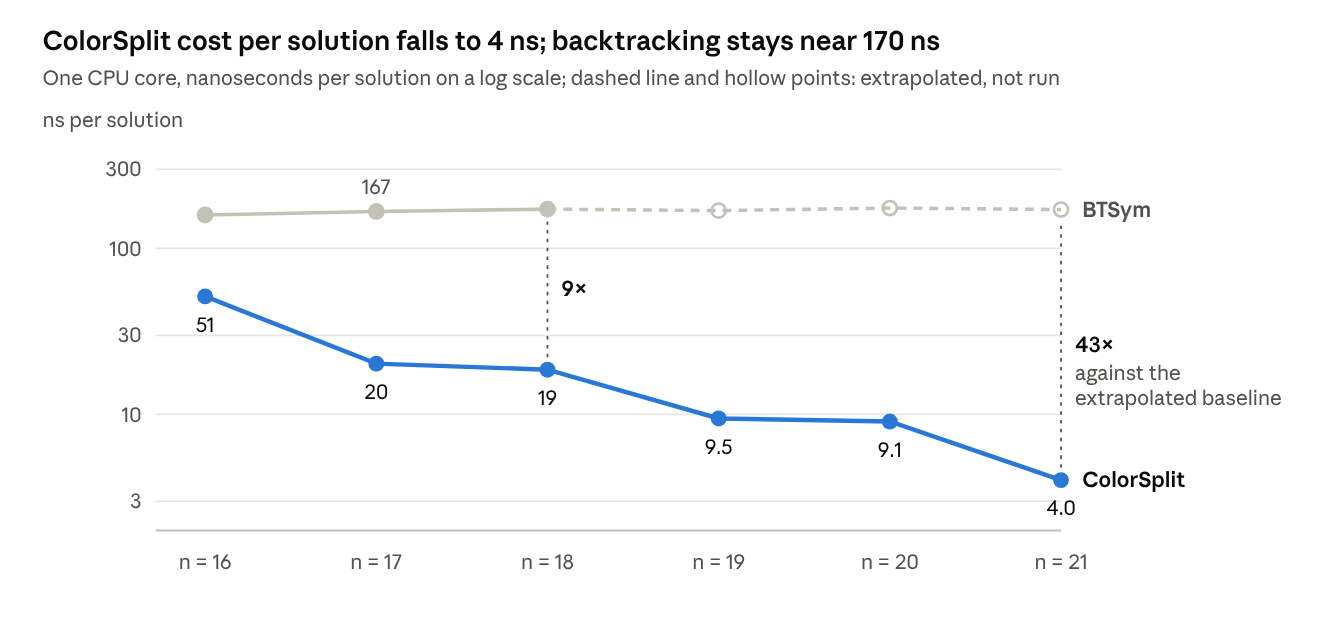
\includegraphics[width=\textwidth]{figs/fig7.png}
\caption{Cost per solution on one CPU core, from the times in the table above}\label{fig:7}
\end{figure}

In our measurements backtracking pays a roughly constant 160 to 175 ns per solution, while ColorSplit's cost per solution falls with n, because solutions are counted in bulk (Figure 7). ColorSplit's running time grows by a factor of 2.5 to 4 on steps to odd n and 6 to 8 on steps to even n, where transposition saves less.

Figure 8 shows the GPU times on a single NVIDIA RTX PRO 6000 Blackwell Server Edition (188 SMs, 96 GB, 600 W power limit) in Google Colab; at the time of writing the runtime provided NVIDIA driver 580.82.07 and CUDA 13.0 (nvcc 13.0.88). Q(22) and Q(24) were computed with the first version of the kernel, Q(25) with the second version before tuning, and Q(23), Q(26) and Q(27) with the tuned second version; tuning cut the time for Q(23) from 3.2 to 2.5 minutes. Q(28) was computed with the current version (Section 6), saving a checkpoint every 8 chunks. Each GPU time is from a single run.

\begin{figure}[htbp]\centering
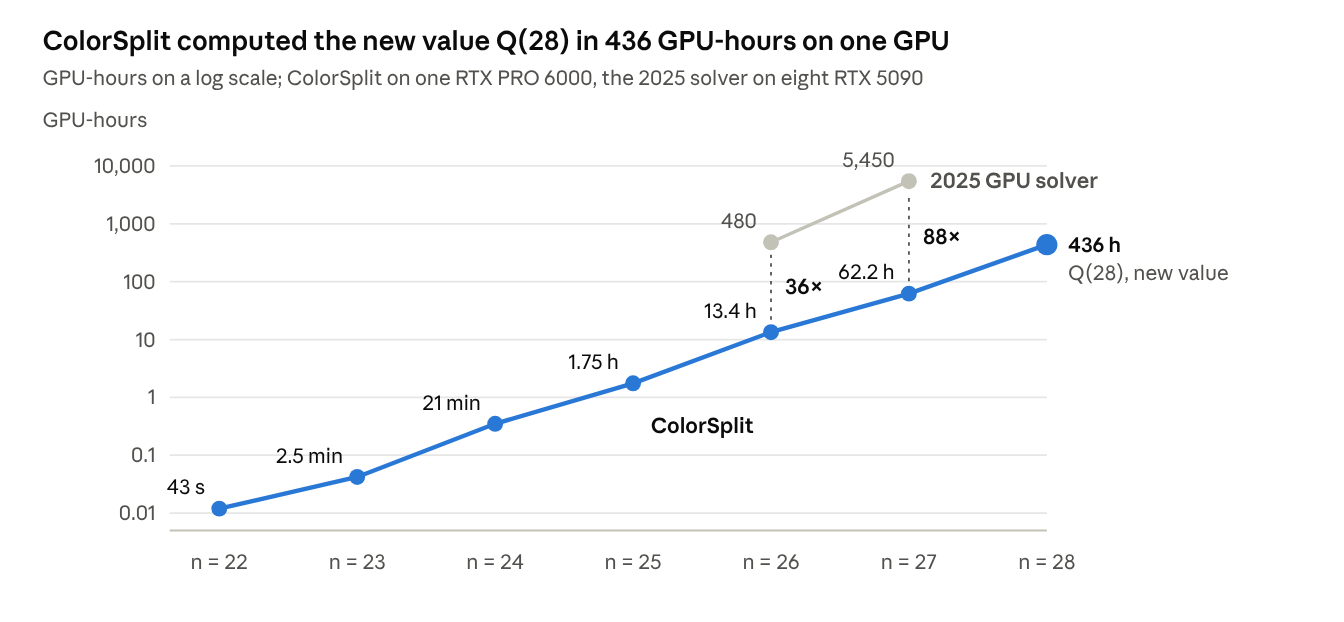
\includegraphics[width=\textwidth]{figs/fig8.png}
\caption{GPU-hours per value of Q(n): our runs on Google Colab; the 2025 solver as reported in arXiv:2511.12009}\label{fig:8}
\end{figure}

For comparison, the 2025 GPU solver needed 2.5 days on eight RTX 5090 GPUs for Q(26), about 480 GPU-hours [arXiv:2511.12009]. ColorSplit used 13.4 GPU-hours of one RTX PRO 6000, a card of the same Blackwell generation with about 10\% more streaming multiprocessors (188 against 170): about 36 times fewer GPU-hours. For Q(27) that solver needed 28.4 days on eight GPUs, about 5450 GPU-hours; ColorSplit recomputed Q(27) in 62.2 GPU-hours, about 88 times fewer. These ratios compare running times reported for different hardware and software; they are a rough comparison of total resources, not a controlled benchmark. To our knowledge that solver has not reported Q(28); its authors projected about 11 months on eight RTX 5090 GPUs for it, roughly 64,000 GPU-hours.

Our Q(27) run took 2.74 days of wall time because the cloud session was interrupted several times; 3.6 hours of work lost in the first interruption, before the checkpoint file was made robust, are not counted. Our Q(28) run took 436.4 hours of computation, 18.2 days, over several cloud sessions, each resuming from the checkpoint file; at 8.9 compute units per hour that is about 3,900 units, roughly CAD 520. Q(26) cost about 120 cloud compute units, roughly CAD 16. On rented CPUs, eight virtual cores computed Q(23) in 72 minutes (C version) and Q(24) in 22 hours (Java version).

On this GPU the step from Q(25) to Q(26) cost a factor of about 9.5 after correcting for later tuning, the step from Q(26) to Q(27) a factor of 4.7, and the step from Q(27) to Q(28) a factor of 7.0, with the faster current kernel for Q(28). The model $\sqrt{Q(n)}$ · 2$^{n}$, with transposition saving a factor of 2 on odd boards and 1.4 on even ones, predicts about 9.1 and 4.5 for the first two steps, in line with the measurements, but 9.4 for the step to Q(28). The measured 7.0 is about 25\% lower, more than the gain of about 8\% we measured for the current kernel at n = 27; we have not isolated the cause. Before the run we had extrapolated 590–690 GPU-hours for Q(28) from the second version of the kernel; the current version needed 436. With a factor of about 4.7 for the next odd step, Q(29) would need roughly 2,000 GPU-hours, about three months of one such GPU. The checkpoint format lets such runs be split over several GPUs with no loss.

\section{What did not help}

In our implementations most ideas for further speedups did not pay off, for one of three reasons: they needed a disjointness test instead of an exact key, they pruned too few branches to pay for their cost per node, or they were not exact. We list them with our measurements; other implementations or combinations of these ideas may do better.

\begin{table}[htbp]\centering\small
\begin{tabularx}{\textwidth}{>{\raggedright\arraybackslash}p{0.27\textwidth}>{\raggedright\arraybackslash}X>{\raggedright\arraybackslash}X}\toprule
Idea & Measured effect & Reason \\\midrule
Second split inside one color (EE + OO, EO + OE, top + bottom, left + right halves) & 1.7 to 20 times slower; with 64-bit bitset joins at best equal to backtracking & the parts share diagonals (Lemma 3), so our joins needed a disjointness test \\
Reusing work between row sets by shifting or sharing common cores & model saves 1.3 to 1.7 times in operations; real code 3 to 9\% slower & in our code, bookkeeping per leaf and per group outweighed the saved enumeration \\
Filtering families of placements related by shifts & wrong answers & shifted placements can differ in having a partner: 1470 mixed families at n = 12 \\
Forward checking on rows and columns & 22 to 39\% fewer nodes, 2.7 to 3 times slower & in our code each check cost more than the branches it removed \\
Radial, sector, vector and weight bounds ("flower" statistics) & under 1\% of nodes, falling with n & no exact linear laws beyond rows and columns for n = 9 to 32 (Lemma 2); the inexact bounds cut few branches \\
Inclusion–exclusion and graphlet counts & exact, but 60 to 1600 times slower at n ≤ 13 & in our formulation the coefficients up to order n/2 cost as much as counting itself \\
Diagonal-first (rotated) enumeration of color parts & 7 times slower & probably because rows are fixed in a part, which row-based enumeration uses directly \\
Rewriting the CPU recursion with an explicit stack & 7 to 16\% slower in Java & probably because the JIT compiler keeps recursive state in registers \\
More classes of diagonals: r + c and r − c taken mod 3 or mod 4 instead of mod 2 (a question from T. B. Preußer) & no new counting law; even a perfect filter on row sets would save under 2\% of the work at n = 17; a nested split inside each color by mod 4 needed 4.6 to 5.6 times more search steps than direct enumeration at n = 12 to 16 & only mod 2 makes r + c and r − c agree, so with more classes the parts share diagonals (Lemma 3) and their join needs a disjointness test; finer classes add no linear law (Lemma 2) \\
\bottomrule
\end{tabularx}
\end{table}

Two patterns stood out. A static order that puts the most constrained lines first beat every dynamic filter we tried: center-out rows gained 10 to 20\% at no cost per node, and a short-diagonals-first order gave 1.6 to 1.9 times on a related problem. And an oracle that knows which 8-row prefixes complete removes two thirds of backtracking nodes at n = 14, while the cheap tests we tried caught only 4 to 7\%; this large gap is consistent with completion being NP-complete [Gent et al. 2017].

\section{Discussion and outlook}

In our measurements the color decomposition changes how the cost grows with n, not just a constant factor: the cost per solution falls with n instead of staying flat. Together with the symmetries and the GPU implementation, this brings Q(26) from months of FPGA time or days of eight GPUs to half a day on one card, and it made the previously unknown Q(28) a computation of 18 days on one card.

We do not know how far the method can be improved. Several times during this work the code seemed close to its limit, and each time further gains were found: the center-out row order, the compact table and the nested mirror all came after such a point. Lemma 3 rules out only one kind of refinement, a second split of the squares with an exact key; decompositions of other kinds, and better tables, row orders or symmetries, remain open. The reserves we can see now are transposition on even boards, which saves a factor of 1.4 out of a possible 2; sharing work between row sets, which saved operations in our models but not yet time in our code (Section 9); and memory access on the GPU, which dominates on large boards.

Our next steps:

\begin{enumerate}
\item{} Q(27): our value 234,907,967,154,122,528 is, to our knowledge, the third independent computation of this value, after the Q27 project of 2016 [Preußer and Engelhardt 2017] and the GPU solver of 2025 [arXiv:2511.12009], and the first by a method that does not enumerate solutions one by one. We call it independent because it shares neither code nor method with the other two.
\item{} Q(28) = 2,564,269,152,506,723,832 is new, and it should be confirmed independently. The published partial sums let anyone recompute any part of it, and we welcome such checks. It still fits in a signed 64-bit integer, with a margin of a factor of 3.6, which likely makes 28 the last such case.
\item{} Q(29) is about 11 times larger, so the total no longer fits in 64 bits (each chunk sum still does), and by our estimate it needs about 2,000 GPU-hours, roughly three months of one GPU. The 4096 independent, individually checkable chunks make it a good fit for volunteer or cluster computing.
\end{enumerate}

The code for CPUs and GPUs, the checkpoint files of our Q(27) and Q(28) runs with all 4096 partial sums each, and the scripts that check and merge checkpoint files are released with this paper at \href{https://github.com/SergeyChere/colorsplit-nqueens}{github.com/SergeyChere/colorsplit-nqueens}, so that every chunk of both results can be recomputed independently.

\section{Author contributions and use of AI}

All of this research was done with the help of Claude, an AI model developed by \href{https://www.anthropic.com}{Anthropic}, in September and October 2026. In short, the paper reports the author's ideas, checked and implemented with Claude, and the author's own runs on large boards.

\begin{itemize}
\item{} \textbf{Ideas.} The author set the goal and the direction of the research and proposed its central ideas: splitting the board by color (found independently; for bishops the color split goes back to Arshon, see Section 2), the parity law on rows, the mirror reductions for odd boards including the nested mirror, the center-out row order, and checking chunks by recomputing them with the opposite table side.
\item{} \textbf{Large computations.} The author ran all computations for n ≥ 22 by hand, on rented CPU servers and on cloud GPUs, watched and restarted them, and checked their results.
\item{} \textbf{Implementation and testing.} Claude wrote the Java, C and CUDA programs, ran the experiments and benchmarks up to n = 21, tested each idea against data and reported which ones failed and why, proposed several implementation techniques such as the compact table and the design of the GPU kernel, and drafted the text and the figures of this paper.
\end{itemize}

The author reviewed the text and the results and takes full responsibility for the paper.

\section*{Acknowledgments}
\addcontentsline{toc}{section}{Acknowledgments}

We thank Thomas B. Preußer for reading a draft of this paper, for his comments on its presentation, and for the question about more classes of diagonals discussed in Section 9.

\section*{References}\small\raggedright
\addcontentsline{toc}{section}{References}

\begin{itemize}
\item{} [Abramson and Yung 1989] B. Abramson, M. Yung. Divide and conquer under global constraints: a solution to the N-queens problem. Journal of Parallel and Distributed Computing 6, 649–662, 1989.
\item{} [Arshon 1936] S. E. Arshon. Solution of a combinatorial problem (in Russian). Matematicheskoe Prosveshchenie 8, 24–29, 1936.
\item{} [arXiv:2511.12009] G. Yao, Y. Li. High-Performance N-Queens Solver on GPU: Iterative DFS with Zero Bank Conflicts, 2025. \href{https://arxiv.org/abs/2511.12009}{arxiv.org/abs/2511.12009}
\item{} [Bell and Stevens 2009] J. Bell, B. Stevens. A survey of known results and research areas for n-queens. Discrete Mathematics 309(1), 1–31. \href{https://doi.org/10.1016/j.disc.2007.12.043}{doi:10.1016/j.disc.2007.12.043}
\item{} [Chaiken et al. 2014] S. Chaiken, C. R. H. Hanusa, T. Zaslavsky. A q-Queens Problem. I. General Theory. Electronic Journal of Combinatorics 21(3), \#P3.33, 2014. \href{https://arxiv.org/abs/1303.1879}{arXiv:1303.1879}
\item{} [Chaiken et al. 2020] S. Chaiken, C. R. H. Hanusa, T. Zaslavsky. A q-Queens Problem. V. Some of Our Favorite Pieces: Queens, Bishops, Rooks, and Nightriders. Journal of the Korean Mathematical Society 57(6), 1407–1433, 2020. \href{https://arxiv.org/abs/1609.00853}{arXiv:1609.00853}
\item{} [Gent et al. 2017] I. P. Gent, C. Jefferson, P. Nightingale. Complexity of n-Queens Completion. Journal of Artificial Intelligence Research 59, 815–848. \href{https://doi.org/10.1613/jair.5512}{doi:10.1613/jair.5512}
\item{} [Kise et al. 2004] K. Kise, T. Katagiri, H. Honda, T. Yuba. Solving the 24-queens Problem using MPI on a PC Cluster. Technical Report UEC-IS-2004-6, University of Electro-Communications.
\item{} [Kluev] E. Kluev. N-Queens-Count-Sol: counting n-queens solutions by joining partial solutions of the four quarters of the board. Source code, \href{https://github.com/EvgenyKluev/N-Queens-Count-Sol}{github.com/EvgenyKluev/N-Queens-Count-Sol}
\item{} [Kotěšovec 2013] V. Kotěšovec. Non-attacking chess pieces (chess and mathematics). 6th edition, self-published, Prague, 2013.
\item{} [Nielsen 2026] H. Nielsen. The n-queens solution count Q(n) is divisible by 4. \href{https://arxiv.org/abs/2601.05856}{arXiv:2601.05856}
\item{} [OEIS A000170] Number of ways of placing n nonattacking queens on an n × n board. The On-Line Encyclopedia of Integer Sequences. \href{https://oeis.org/A000170}{oeis.org/A000170}
\item{} [Preußer et al. 2009] T. B. Preußer, B. Nägel, R. G. Spallek. Putting Queens in Carry Chains. Technical Report TUD-FI09-03, Fakultät Informatik, TU Dresden, 2009.
\item{} [Preußer and Engelhardt 2017] T. B. Preußer, M. R. Engelhardt. Putting Queens in Carry Chains, No. 27. Journal of Signal Processing Systems 88(2), 2017. \href{https://doi.org/10.1007/s11265-016-1176-8}{doi:10.1007/s11265-016-1176-8}; code: \href{https://github.com/preusser/q27}{github.com/preusser/q27}
\item{} [Richards 1997] M. Richards. Backtracking algorithms in MCPL using bit patterns and recursion. Technical Report UCAM-CL-TR-433, University of Cambridge Computer Laboratory, July 1997. \href{https://www.cl.cam.ac.uk/techreports/UCAM-CL-TR-433.html}{cl.cam.ac.uk/techreports/UCAM-CL-TR-433}
\item{} [Simkin 2023] M. Simkin. The number of n-queens configurations. Advances in Mathematics 427, 109127. \href{https://doi.org/10.1016/j.aim.2023.109127}{doi:10.1016/j.aim.2023.109127}; \href{https://arxiv.org/abs/2107.13460}{arXiv:2107.13460}
\end{itemize}

